%!TEX root =  ../main.tex

\objective{Find higher derivatives of functions, apply and produce their graphs}


\index{Concavity}
The first derivative of a function tell you the slope of the graph at any point.  When the
derivative function is positive, the original graph slopes up.  When it is negative the original
graph slopes down.  When it is zero, the original graph is flat.  

Could you graph the original function if you were given the derivative?  Well, you wouldn't 
know where to start, but once you picked a beginning, your slope would make it clear
where to go from there.  Practice staying within the graphical realm, drawing the derivative
of a given function, or a possible function given its derivative graph.


\subsection{Second Derivatives}
But what about the derivative of the derivative?
The slope of the slope is the rate of change, or acceleration.  Think about what happens when
you accelerate, even if you are traveling backwards at first: your velocity becomes more and more
positive.  On the other hand, deceleration means slowing down and quickly traveling backwards more and
more quickly.

\begin{figure}
\begin{centering}
\begin{tabular}{ |c|c|l| }
\hline
$f'(x)$ & $f''(x)$ & $f(x)$ \\ \hline \hline
\multirow{3}{*}{ + } & + & right side of a valley \\ \cline{2-3}
 & 0 & top of a peak \\ \cline{2-3}
 & - & left side of a mountain \\ \hline
\multirow{3}{*}{ 0 } & + & end of a valley, start of a peak \\ \cline{2-3}
 & 0 & plateau \\ \cline{2-3}
 & - & end of a peak, start of a valley \\ \hline
\multirow{3}{*}{ - } & + & ride side of a valley \\ \cline{2-3}
 & 0 & bottom of a valley \\ \cline{2-3}
 & - & right side of a peak \\
\hline
\end{tabular}
\caption{Relating first and second derivative signs to a graph}
\end{centering}
\end{figure}


Most of these behaviors can be seen in figure ...  The solid curve is $f(x)=\frac{1}{6}x^6
-2x^4+8x^2-20$.  The dashed curve is $f'(x)$ and the dotted is $f''(x)$.

\begin{figure}\label{derivativesigns}
\begin{centering}
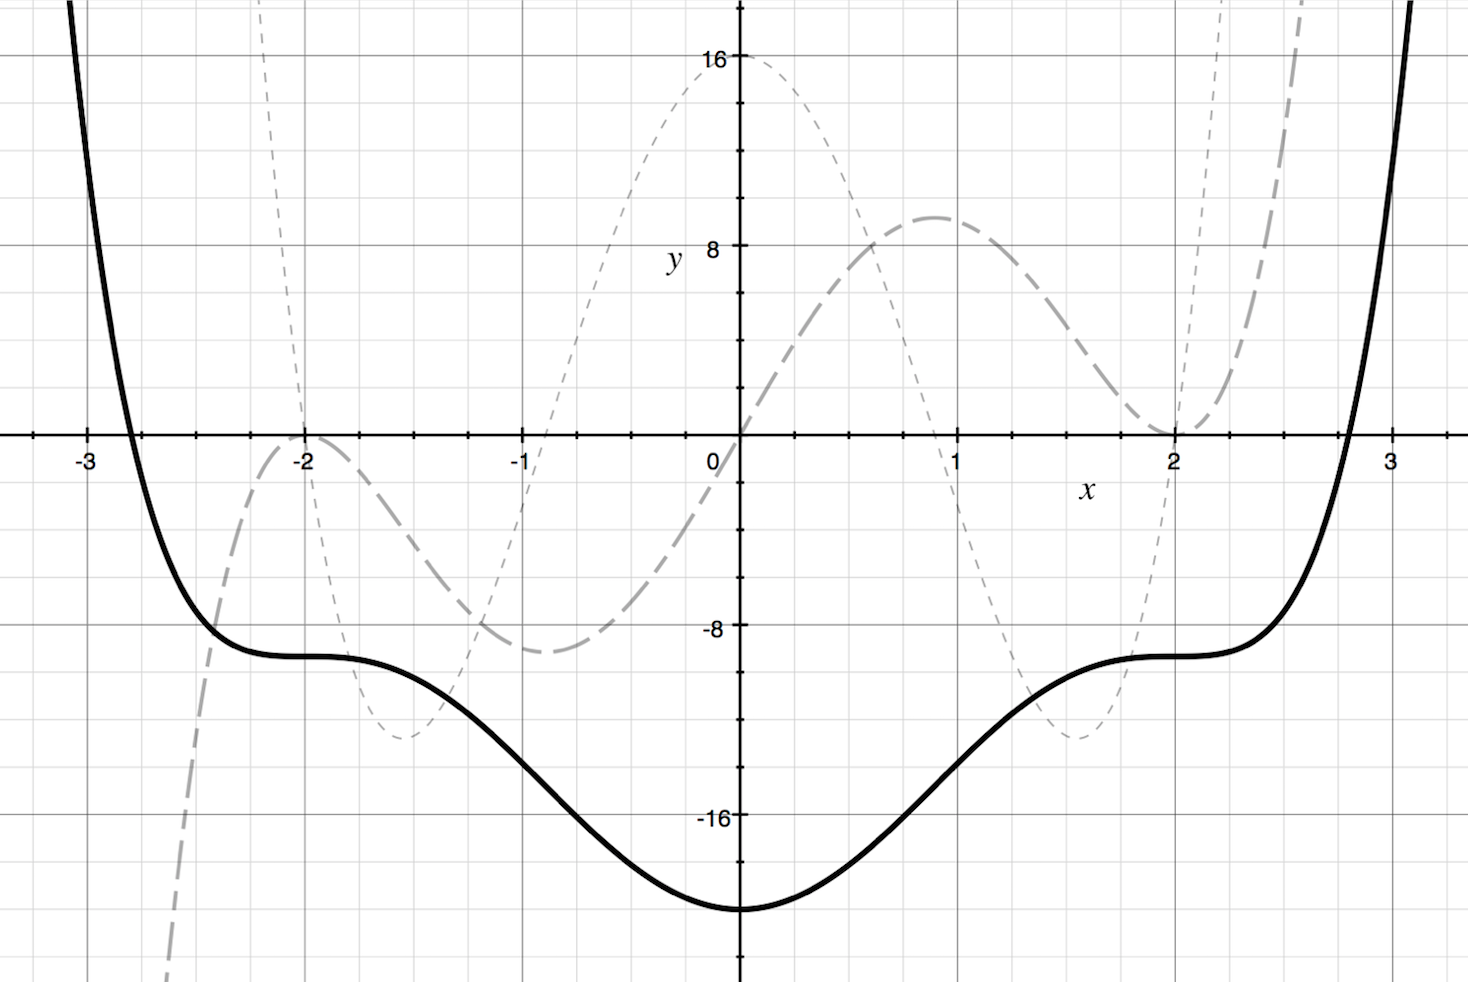
\includegraphics[width=\textwidth]{derivativesigns}
\caption{A function with inflection and turning points}
\end{centering}
\end{figure}

